\documentclass[UTF8, aspectratio=169,10pt]{beamer}% ratio:aspectratio=169,1610,43,32
\hypersetup{pdfpagemode=FullScreen}
\setbeamersize{text margin left=0.05\paperwidth, text margin right=0.05\paperwidth}
%\usepackage{pgfpages}
%\pgfpageslogicalpageoptions{1}{border code=\pgfstroke}
%\pgfpageslogicalpageoptions{2}{border code=\pgfstroke}
%\pgfpageslogicalpageoptions{3}{border code=\pgfstroke}
%\pgfpageslogicalpageoptions{4}{border code=\pgfstroke}
%\pgfpagesuselayout{4 on 1}[a4paper,landscape,border shrink=5mm]

%==============xeCJK settings============================================================%
\usepackage{xeCJK}
\xeCJKsetup{CJKmath=true}
\xeCJKsetup{CheckSingle=true,PlainEquation=true}
\xeCJKsetup{AutoFakeBold}
\xeCJKsetup{AutoFakeSlant}
\xeCJKsetup{PunctStyle=CCT}
\xeCJKsetup{AllowBreakBetweenPuncts=true}


\usefonttheme{serif}
\setCJKmainfont[Mapping=fullwidth-stop]{华文楷体}
\setCJKsansfont[Mapping=fullwidth-stop]{微软雅黑}
\setCJKmonofont[Mapping=fullwidth-stop]{等线}

\setmainfont[Mapping=tex-text]{XITS}
\setsansfont[Mapping=tex-text]{Arial}
\setmonofont[Mapping=tex-text]{Courier New}

\XeTeXlinebreaklocale "zh"
\XeTeXlinebreakskip = 0pt plus 1pt minus 0.1pt

\usepackage{indentfirst}
\setlength{\parindent}{2em}
\linespread{1.15}

%==============Packages=======================================================%

\usepackage{cquptcolor}
\usepackage{fontawesome}
\usepackage{multicol}
\usepackage{unicode-math}
\usepackage{fontspec}
\usepackage{boldline}
\usepackage{svg}
\usepackage{pifont}
\usepackage{colortbl}
\usepackage{cleveref} % 加载 cleveref 宏包
\usepackage{comment}
\usepackage{graphicx}
\usepackage{epstopdf}
\usepackage{ifpdf}
\usepackage{subcaption}
\usepackage{animate}
\usepackage{tikz}
\usepackage{bm}
\usepackage{hyperref}\hypersetup{CJKbookmarks=true}
\usepackage{url}
\usepackage{extarrows}
\usepackage{amsmath}
\usepackage{amsthm}
\usepackage{amssymb}
\usepackage{ytableau}
\usepackage{amsfonts,amsmath,amssymb,amscd,bm}
\usepackage{longtable}
\usepackage{booktabs} % for much better looking tables
\usepackage{cite} % reference
\usepackage{array} % for better arrays (eg matrices) in maths
%\usepackage{paralist} % very flexible & customisable lists (eg. enumerate/itemize, etc.)
\usepackage{verbatim} % adds environment for commenting out blocks of text & for better verbatim
% These packages are all incorporated in the memoir class to one degree or another...
\usepackage{threeparttable}
\usepackage{cases} %equation set
\usepackage{multirow} %use table
\usepackage{enumerate}
\usepackage{algorithm}
\usepackage{pifont}
\usepackage{algorithmic}
\usepackage{xcolor}
% \usepackage{caption}
\usepackage{xunicode,xltxtra}
\usepackage{stackengine}
\usepackage{kbordermatrix}
\usepackage{graphicx}
\usepackage{tabularx}
\usepackage{booktabs} % 提供三线表样式
\usepackage{subcaption}
\usepackage{ctex}
% 配置 cleveref,使其使用中文前缀
\crefname{figure}{图}{图}
\crefname{subfigure}{图}{图}
\crefname{table}{表}{表}

%==============Figs,Tabs,Eqs settings======================================================%


\graphicspath{{fig/}}
\numberwithin{equation}{section}
\numberwithin{figure}{section}
\numberwithin{table}{section}


%===================Newdefs=============================================================%
\def\pf{\noindent {\textbf{证明.} \hskip 0.5em}}
\def\jie{\noindent {\textbf{解.} \hskip 0.5em}}
\def\ps{\mathrm{ps}}
\def\blue{\textcolor{blue}}
\def\red{\textcolor{red}}
\def\dui{{\LARGE\setmainfont{Linux Libertine O}\red{\symbol{"2714}}}}
\def\cuo{{\LARGE\setmainfont{Linux Libertine O}\red{\symbol{"2718}}}}
\def\finger{\cquptgreen\faHandORight~~}
\def\que{\cquptgreen\faQuestionCircle}
\def\T{{\rm T}}
\def\F{{\rm F}}
\def\opxy{\langle x, y\rangle}
\def\kongbai{\usebackgroundtemplate{}}
\def\dom{{\rm dom}}
\def\ran{{\rm ran}}
\def\fld{{\rm fld}}




\newcommand\cclap[3][0pt]{\stackengine{0pt}{#3}{\kern#1#2}{O}{c}{F}{F}{L}}
\def\notr{\cclap{$/$}{$R$}}


\newcommand{\alertg}[1]{\cquptgreen{\textbf{#1}}}

%===================Thm's environment=============================================================%

\theoremstyle{definition}
\newtheorem{thm}{定理}[section]
\newtheorem{cor}[thm]{推论}
\newtheorem{lem}[thm]{引理}
\newtheorem{prop}[thm]{性质}
\newtheorem{claim}[thm]{声明}
\newtheorem{defi}{}[section]
\newtheorem{rem}{注}[section]
\newtheorem{exam}{例}[section]
\newtheorem{ack}{致谢}[section]
\newtheorem{conj}{猜想}[section]
\newtheorem{ques}[conj]{问题}

\makeatletter
\newtheorem*{rep@theorem}{\rep@title}
\newcommand{\newreptheorem}[2]{%
\newenvironment{rep#1}[1]{%
 \def\rep@title{#2 \ref{##1}}%
 \begin{rep@theorem}}%
 {\end{rep@theorem}}}
\makeatother
\newreptheorem{exam}{例}
\newreptheorem{thm}{定理}
%\newtheorem{thm}{Theorem}[section]
%\newtheorem{cor}[thm]{Corollary}
%\newtheorem{lem}[thm]{Lemma}
%
%\newtheorem{prop}{Proposition}[section]
%\newtheorem{defi}{Definition}[section]
%\newtheorem{rem}{Remark}[section]
%\newtheorem{property}{Property}[section]
%\newtheorem{exam}{Example}[section]
%\newtheorem{conj}{Conjecture}[section]
%\setlength{\cftbeforesecskip}{10pt}


%===================Title and author infos=============================================================%
%====the index of Chapter==%%
\def\chapindex{4}          %%
%==========================%%

\title[基于局部代理模型的图神经网络可解释性研究]
{基于局部代理模型的图神经网络可解释性研究 \\[6pt]
\normalsize{Enhancing Explainability of Graph Neural Networks Using Local Proxy Model}}


\author[王以可]
{
	汇报人: 王以可\inst{1} \and
	导师: 刘立~~副教授\inst{2}
}
\institute[2022214508@stu.cqupt.edu.cn]
{
	\inst{1} 2022214508@stu.cqupt.edu.cn \and
	\inst{2} liliu@cqupt.edu.cn
}

\date[\chtoday]{重庆邮电大学~~计算机学院\\[3pt]\chtoday}

%\date[更新于~~\chtoday]{重庆邮电大学~~理学院\\[3pt]更新于~~\chtoday}
%=====================Main body===============================================================================%
% 设置目录深度为1,只显示章节和节
\setcounter{tocdepth}{2}
\begin{document}

{
\usebackgroundtemplate{}
\begin{frame}[plain]
  \titlepage
\end{frame}
}


% 主目录页
\begin{frame}
	\frametitle{目~~录}
	\renewcommand{\baselinestretch}{0.75}\normalsize
	\tableofcontents
\end{frame}

% 在每个子章节开始时显示目录
\AtBeginSubsection[]
{
	\begin{frame}
		\frametitle{\insertsection}
		\renewcommand{\baselinestretch}{1.75}\normalsize
		\tableofcontents[sectionstyle=hide/hide,subsectionstyle=show/shaded/hide]
	\end{frame}
}

%==============================================================================%
\section{选题背景与意义}
\subsection{图神经网络简介}
\begin{frame}{图神经网络简介}
	图神经网络(GNNs)是一种专门用于处理图结构数据的深度学习模型。图结构数据是由节点(vertices)和边(edges)组成的,常见于社交网络、分子结构、交通网络等领域。GNNs的核心思想是通过节点的特征信息和图结构来学习节点的表示(representation)。如\cref{fig:c1}。
\begin{figure}
	\centering
	\begin{subfigure}[b]{0.4\linewidth}
		\centering
		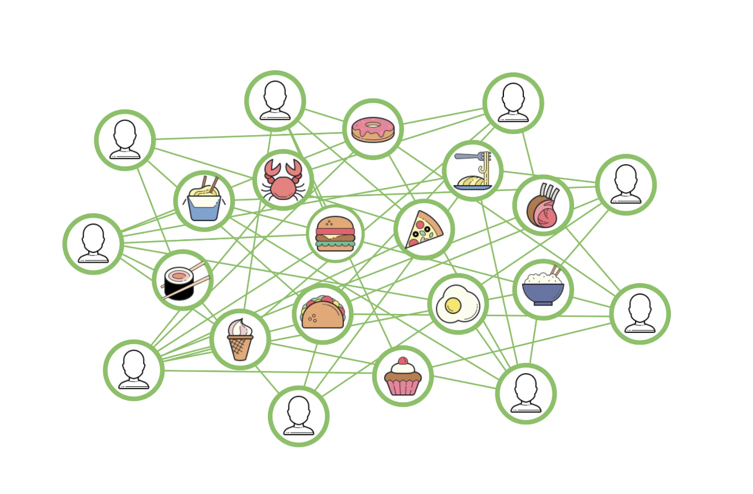
\includegraphics[width=\linewidth]{fig/w1}
		\caption{推荐系统的图模型}
		\label{fig:1}
	\end{subfigure}
\hspace{0.05\linewidth} % 调整这个值来改变间距
	\begin{subfigure}[b]{0.3\linewidth}
		\centering
		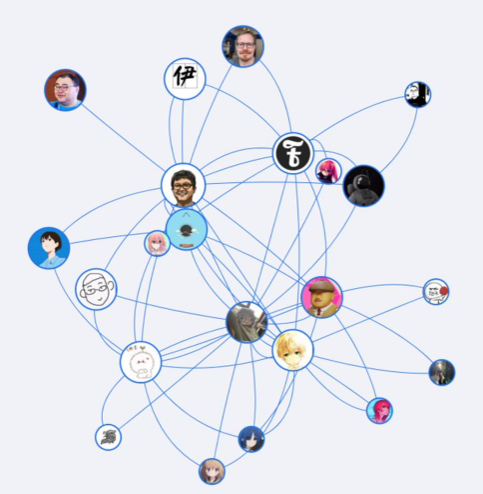
\includegraphics[width=\linewidth]{fig/w2}
		\caption{社交网络的图模型}
		\label{fig:2}
	\end{subfigure}
	\caption{图网络模型结构示例图}
	\label{fig:c1}
\end{figure}

	
\end{frame}
\subsection{图神经网络解释的意义}
\subsubsection{图神经网络解释的意义}

\begin{frame}{图神经网络解释的意义}
	图神经网络(Graph Neural Networks,GNNs)的解释性在于它们能够帮助我们理解为什么模型会做出某些决策,以及模型如何从数据中提取和利用信息。
	\begin{itemize}
	\item \textbf{理解模型决策:}
		解释性可以帮助我们理解模型是如何做出决策的,这对于建立对模型的信任,以及在实际应用中确保模型的公平性和透明度至关重要。
		
		
	\item \textbf{重要决策问题:}
		在某些领域,如医疗和金融,模型必须能够解释其决策过程,以满足法规要求。在医疗领域,模型的决策可能会直接影响到患者的生命。不同的预测会导致不同的治疗方案。
		
	\end{itemize}
	
	
	
\end{frame}


\subsubsection{图神经网络中的代理模型的意义}
\begin{frame}{图神经网络中的代理模型的意义}
	\begin{itemize}

		\item \textbf{简化复杂的拓扑结构} \\
		大图通常具有复杂的拓扑结构,复杂的拓扑结构带来不可避免的噪声,给图神经网络的训练和解释带来挑战。通过使用小图分解和解释大图,可以将复杂问题拆分为易处理的小问题,从而提高模型的可解释性和效率。
		
		\item \textbf{提高模型解释的效率}\\
		在处理具有数万个节点的大规模图时,训练可解释模型(例如PGE,基于图的解释模型)是极具挑战性的,其计算资源和时间开销极为庞大。通过引入代理模型,可以将原始复杂图进行简化,从而显著降低模型训练的复杂度和时间成本。这不仅使得训练过程更加高效,也使得解释生成的速度和质量得到提升。
		

	\end{itemize}
\end{frame}

\section{代理模型的构建}
\subsection{简化原图模型}

\begin{frame}{图的分割方法}
	 简言之,无向图的分割按照切割方式分为边分割(点分区)和点分割(边分区),即切割图时,来确定是切割的点或边。
	 \begin{figure}[htpb]
	 	\centering
	 	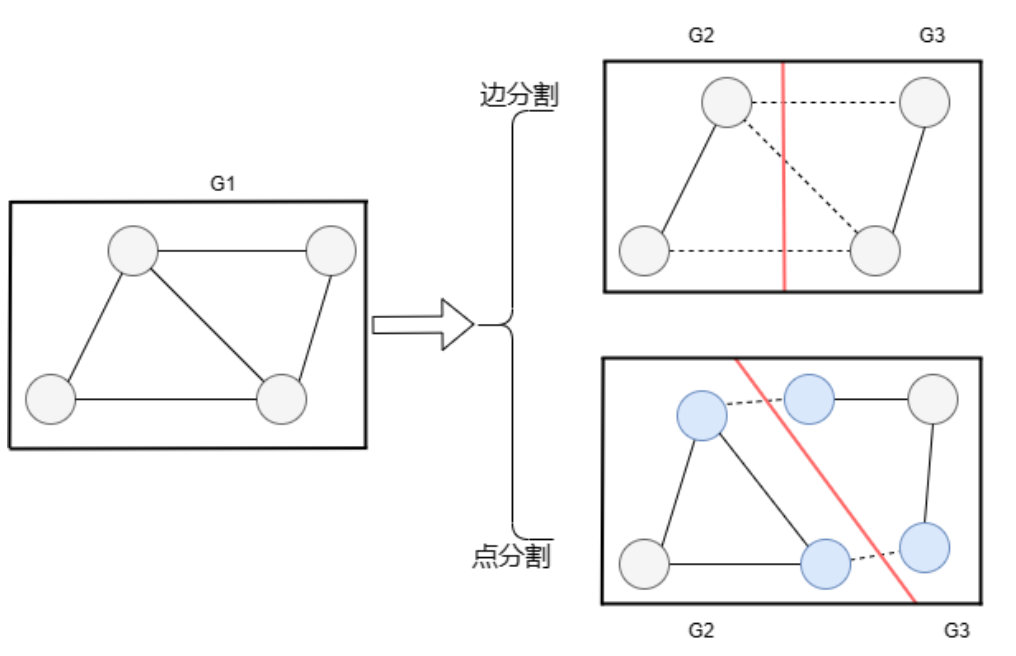
\includegraphics[width=0.5\linewidth]{pic1/a1}
	 	\caption{两种分割方法}
	 	\label{fig:4a}
	 \end{figure}
	
\end{frame}



\begin{frame}{基于社区检测算法的构建}
	我们尝试改进社区发现算法,但发现其时间复杂度较高,对千级节点规模的 Cora 数据集\cref{fig:4}进行切分需要约 45 分钟。此外,社区发现算法更倾向于聚类,而不能很好地保留大图的结构信息。
	\begin{figure}[htpb]
		\centering
		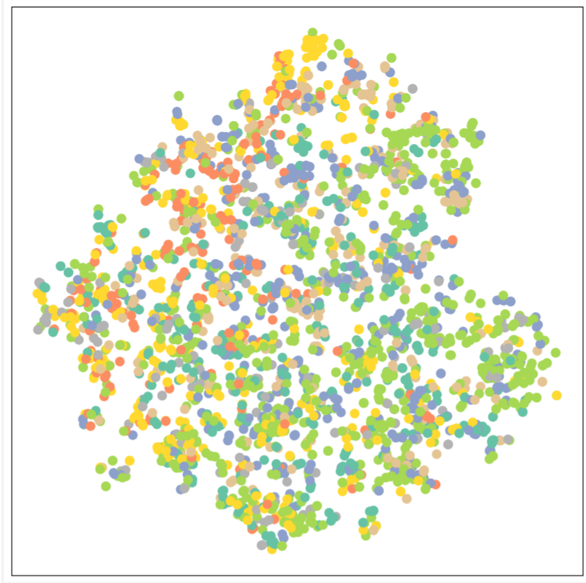
\includegraphics[width=0.33\linewidth]{fig/w3}
		\caption{Cora数据集可视化}
		\label{fig:4}
	\end{figure}
	
	
\end{frame}



\begin{frame}{基于METIS图划分的构建}
	METIS是一种层次化的分割算法(multi-level partitioning),核心思想:对于给定原图结构,持续的降低原图的大小,然后达到一定程度对于缩减后的图结构进行分割,最后将分割后的小图还原成原始的图结构保证每份子图的均衡性。
	\begin{figure}[htpb]
		\centering
		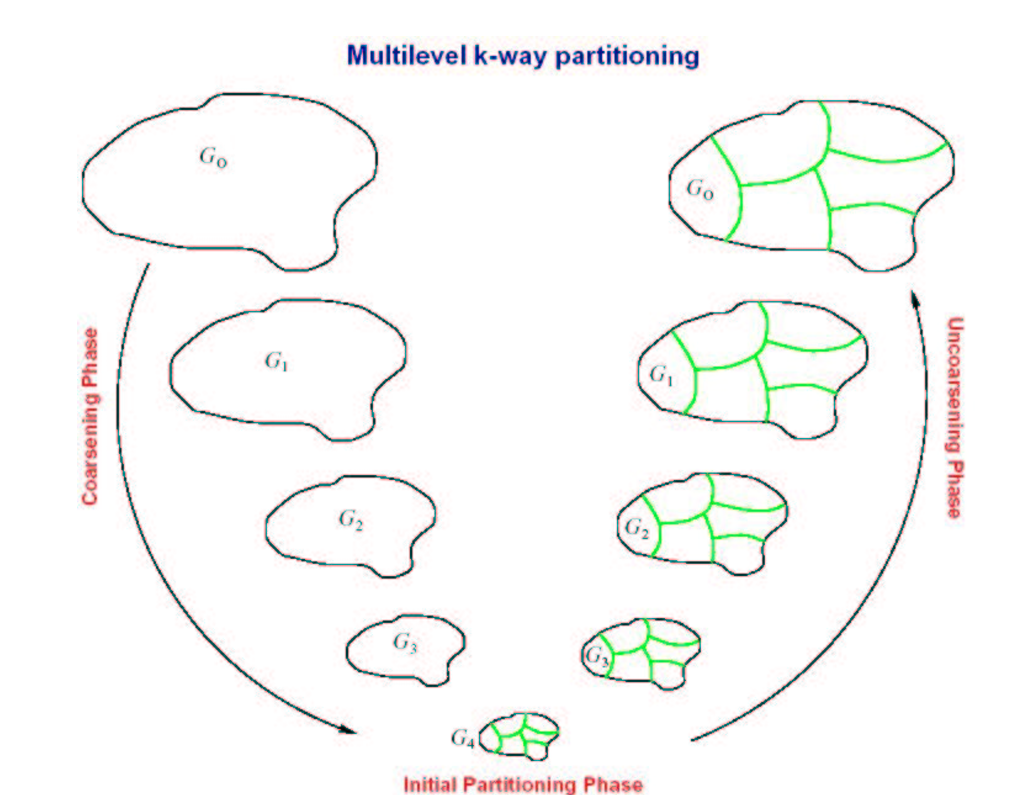
\includegraphics[width=0.4\linewidth]{pic1/a2}
		\caption{METIS图划分}
		\label{fig:4aa}
	\end{figure}
\end{frame}


\begin{frame}{METIS示意图}
	\begin{figure}[htpb]
		\centering
		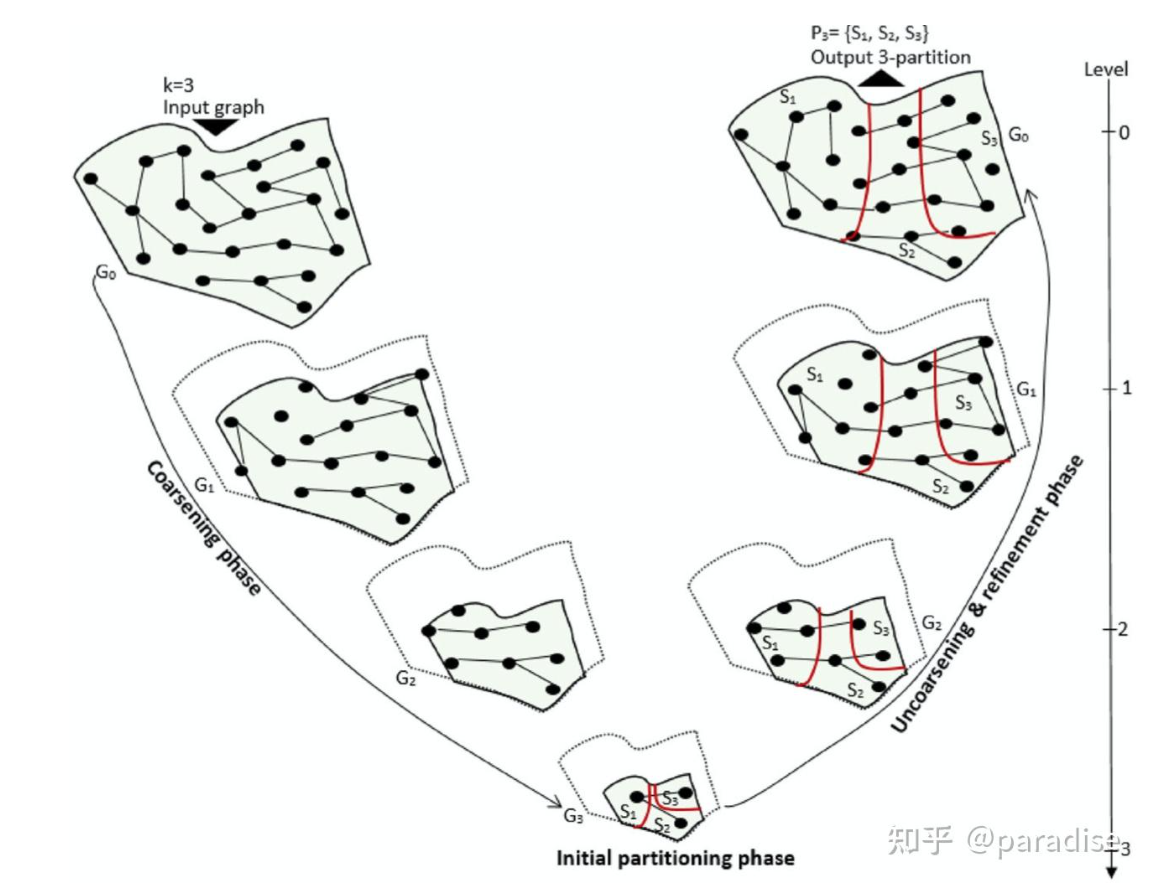
\includegraphics[width=0.6\linewidth]{pic1/a3}
		\caption{METIS图划分}
		\label{fig:4aaa}
	\end{figure}
	
\end{frame}

{
	\kongbai

\begin{frame}{METIS伪代码}
	\begin{figure}[htpb]
		\centering
		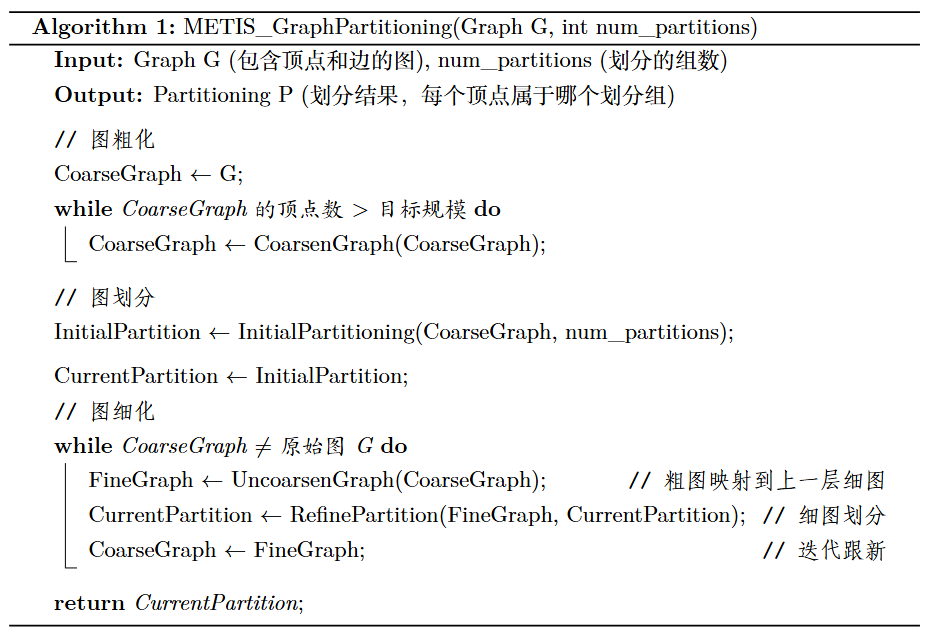
\includegraphics[width=0.7\linewidth]{pic1/a4}
		
		\label{fig:4aawa}
	\end{figure}
\end{frame}



}





\subsection{对原图进行图采样}
\begin{frame}{GraphSaint采样策略}
	它的核心思想是利用概率采样策略,在训练过程中动态生成一系列具备统计代表性的子图样本,然后对这些子图及其节点进行加权归一化,确保训练过程对全图的估计是无偏且高效的。\par
	GraphSaint 提供多种子图采样策略,常用的包括:
	\begin{itemize}
		\item \textbf{节点采样(Node Sampling)}
		\begin{itemize}
			\item 从全图中按照某种概率分布随机选择一组节点,然后取出这些节点及其相连的边形成子图。
			\item 实现简单,对节点特征分布的均匀性有较好的适应性。
		\end{itemize}
		
		\item \textbf{边采样(Edge Sampling)}
		\begin{itemize}
			\item 随机选择一批边,将这些边及其关联的节点作为一个子图。
			\item 对图中边密度的处理更灵活,有时能更好地捕捉图的局部结构特征。
		\end{itemize}
		
		\item \textbf{随机游走采样(Random Walk Sampling)}
		\begin{itemize}
			\item 从一个随机选定的节点出发,在图上进行短程随机游走,将访问到的节点和边作为子图。
			\item 能更好地捕捉图的拓扑结构,适合类社交网络、Web 图等高聚集结构。
		\end{itemize}
	\end{itemize}
\end{frame}




\begin{frame}{GraphSaint+METIS}
METIS 专注于图的分割,但它的分割策略更多是基于局部拓扑信息(如节点和边的分布)进行边分割(Edge Cut),从而减少子图之间的通信开销。\par
\textbf{然而,METIS 划分的结果往往会忽略一些全局图属性,如图的整体结构信息或节点的特征。}\par
GraphSaint 则通过随机采样子图,可以反复从全图中抽取样本,结合全局的统计信息(如节点重要性、特征聚合)来保留全局图的表示能力。

	
\end{frame}



\section{解释模型的应用}
\subsection{解释模型的选取}
\begin{frame}{GNNExplainer}
	GNNExplainer对于解释子图的生成过程是通过优化一个目标函数来实现的,该目标函数旨在最大化GNN的预测与子图结构分布之间的互信息。如\cref{fig:8}。
	\begin{figure}[htpb]
		\centering
		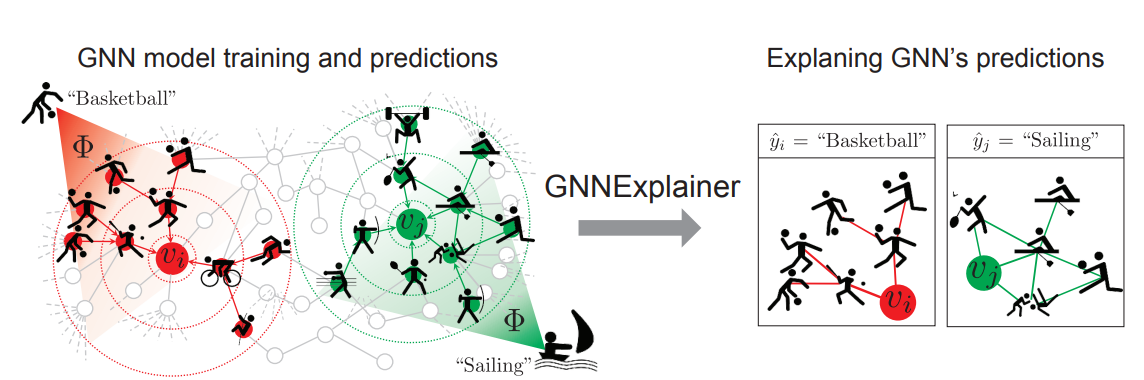
\includegraphics[width=1\linewidth]{fig/w8}
		\caption{Gnne生成解释子图示意图}
		\label{fig:8}
	\end{figure}
	
	
\end{frame}

\begin{frame}{GNNExplainer}
	GNNExplainer 的目标是通过最大化互信息来优化子图和特征掩码,目标函数可以表示为:
	\begin{defi}[GNNExplainer优化函数]
		\begin{equation}\mathcal{L}(M,F)=-\mathbb{E}_{G_S\sim p(G_S|G,M),X_S^F\sim p(X_S^F|X,F)}\left[\log P_\Phi(\hat{Y}|G_S,X_S^F)\right]+\Omega(M,F)\end{equation}
		
		\begin{equation}\mathcal{L}_G(M)=-\mathbb{E}_{G_S\sim p(G_S|G,M)}\left[\log P_\Phi(\hat{Y}|G_S,X)\right]+\Omega_G(M)\end{equation}
		
		\begin{equation}\mathcal{L}_X(F)=-\mathbb{E}_{X_S^F\sim p(X_S^F|X,F)}\left[\log P_\Phi(\hat{Y}|G,X_S^F)\right]+\Omega_X(F)\end{equation}
	\end{defi}
\end{frame}




\subsection{解释子图的生成}
\begin{frame}{大图生成的解释子图}
我们采用两种经典的解释模型,分别在子图和完整图上生成相应的解释子图,并计算解释子图中各节点对目标预测的正确性的影响程度。如\cref{fig:cc2}为GNNE在大图上生成的解释子图对目标节点预测影响度。
	\begin{figure}[h]
		\centering
		\begin{subfigure}[b]{0.40\textwidth}
			\centering
			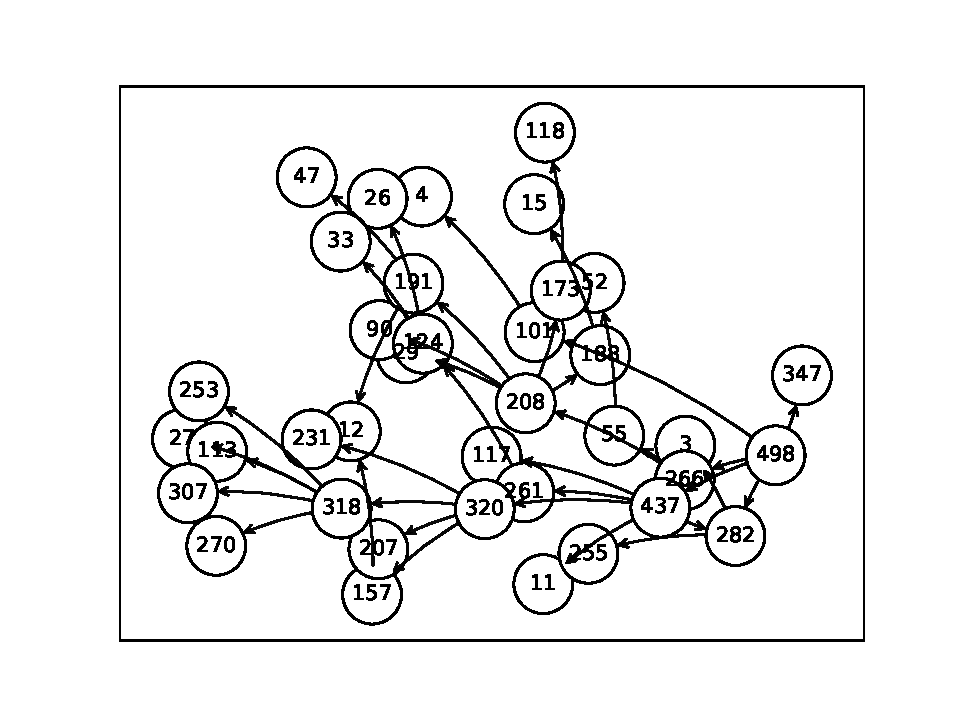
\includegraphics[width=\textwidth]{fig/w91}
			\caption{大图上的解释子图}
			\label{fig:subgraph}
		\end{subfigure}
		\hfill
		\begin{subfigure}[b]{0.40\textwidth}
			\centering
			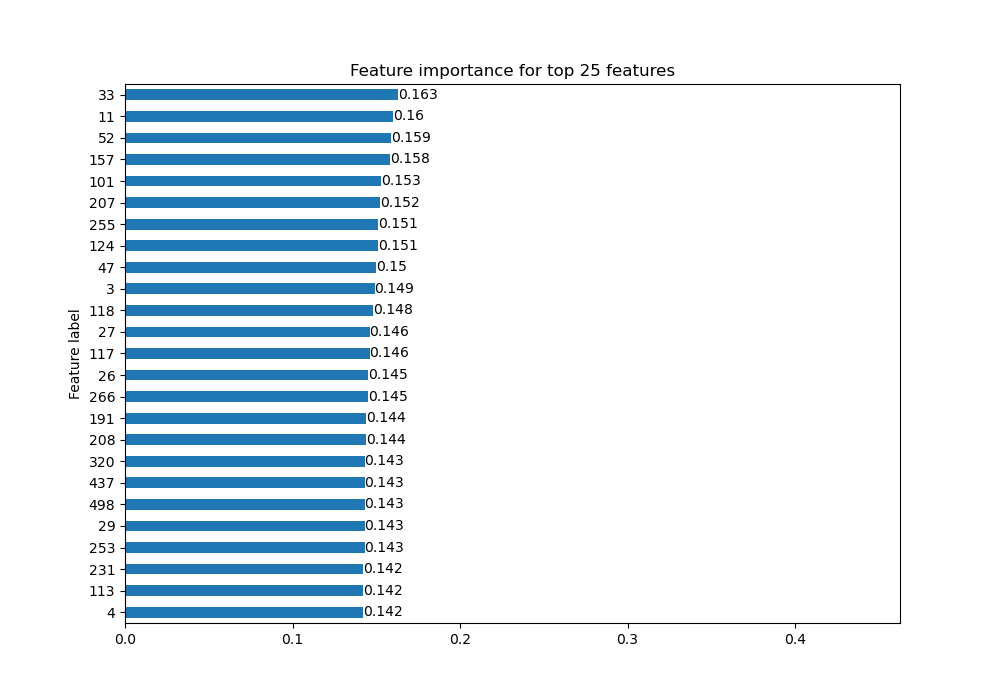
\includegraphics[width=\textwidth]{fig/w92}
			\caption{大图的解释子图对于节点预测影响度排序}
			\label{fig:wholegraph}
		\end{subfigure}
		\caption{大图的解释子图与其影响程度}
		\label{fig:cc2}
	\end{figure}
	
\end{frame}

\begin{frame}{子图生成的解释子图}
	子图上生成的解释子图对目标节点预测影响度如\cref{fig:cc22}。
	\begin{figure}[h]
		\centering
		\begin{subfigure}[b]{0.40\textwidth}
			\centering
			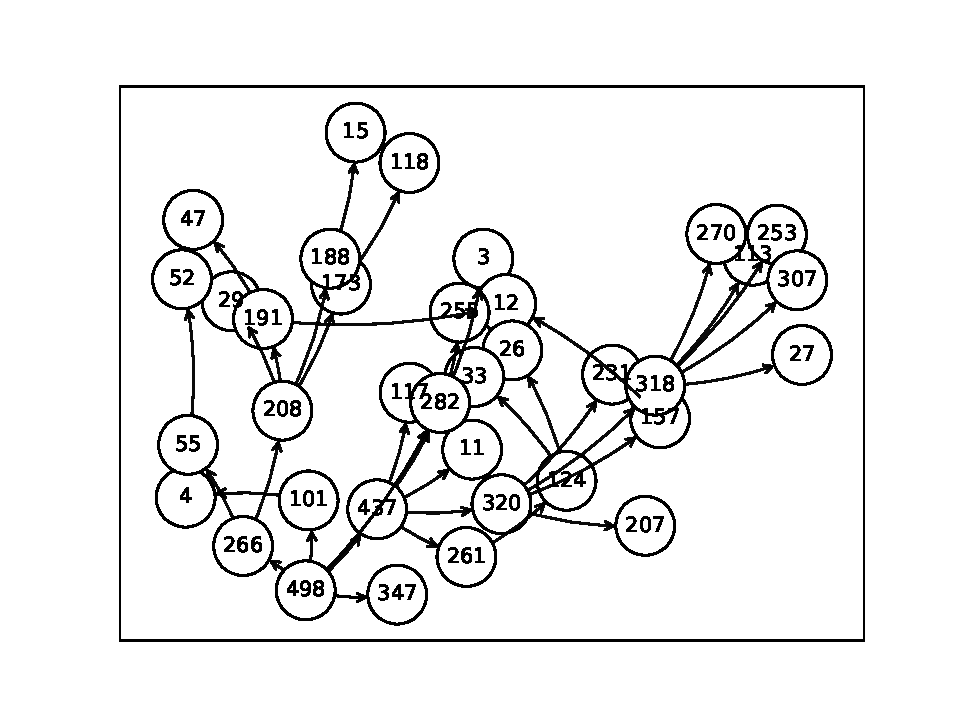
\includegraphics[width=\textwidth]{pic/q1}
			\caption{子图上的解释子图}
			\label{fig:1111}
		\end{subfigure}
		\hfill
		\begin{subfigure}[b]{0.40\textwidth}
			\centering
			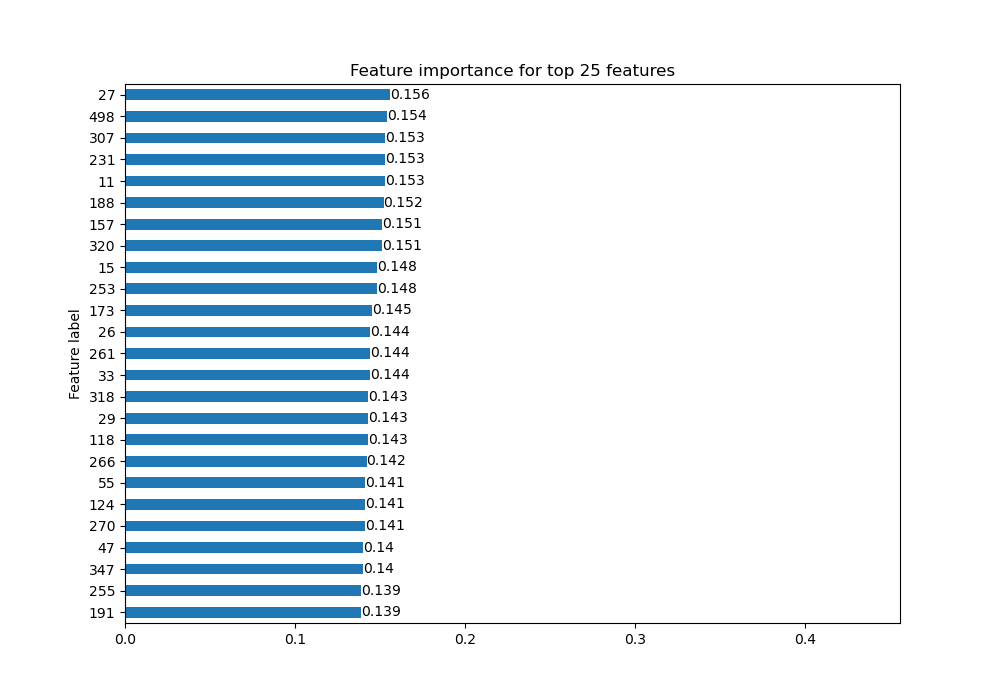
\includegraphics[width=\textwidth]{pic/q2}
			\caption{子图的解释子图对于节点预测影响度排序}
			\label{fig:2222}
		\end{subfigure}
		\caption{子图的解释子图与其影响程度}
		\label{fig:cc22}
	\end{figure}
	
	
	
\end{frame}


\section{解释子图的评价}
\subsection{解释子图的评价方法}
\begin{frame}{评价方法}
	我们通过从大图中移除由大图生成的解释子图和由子图生成的解释子图,来评估这两种解释子图对大图中目标节点预测概率的影响,从而判断解释子图的质量。如\cref{fig:99}。
	
	\begin{figure}[htpb]
		\centering
		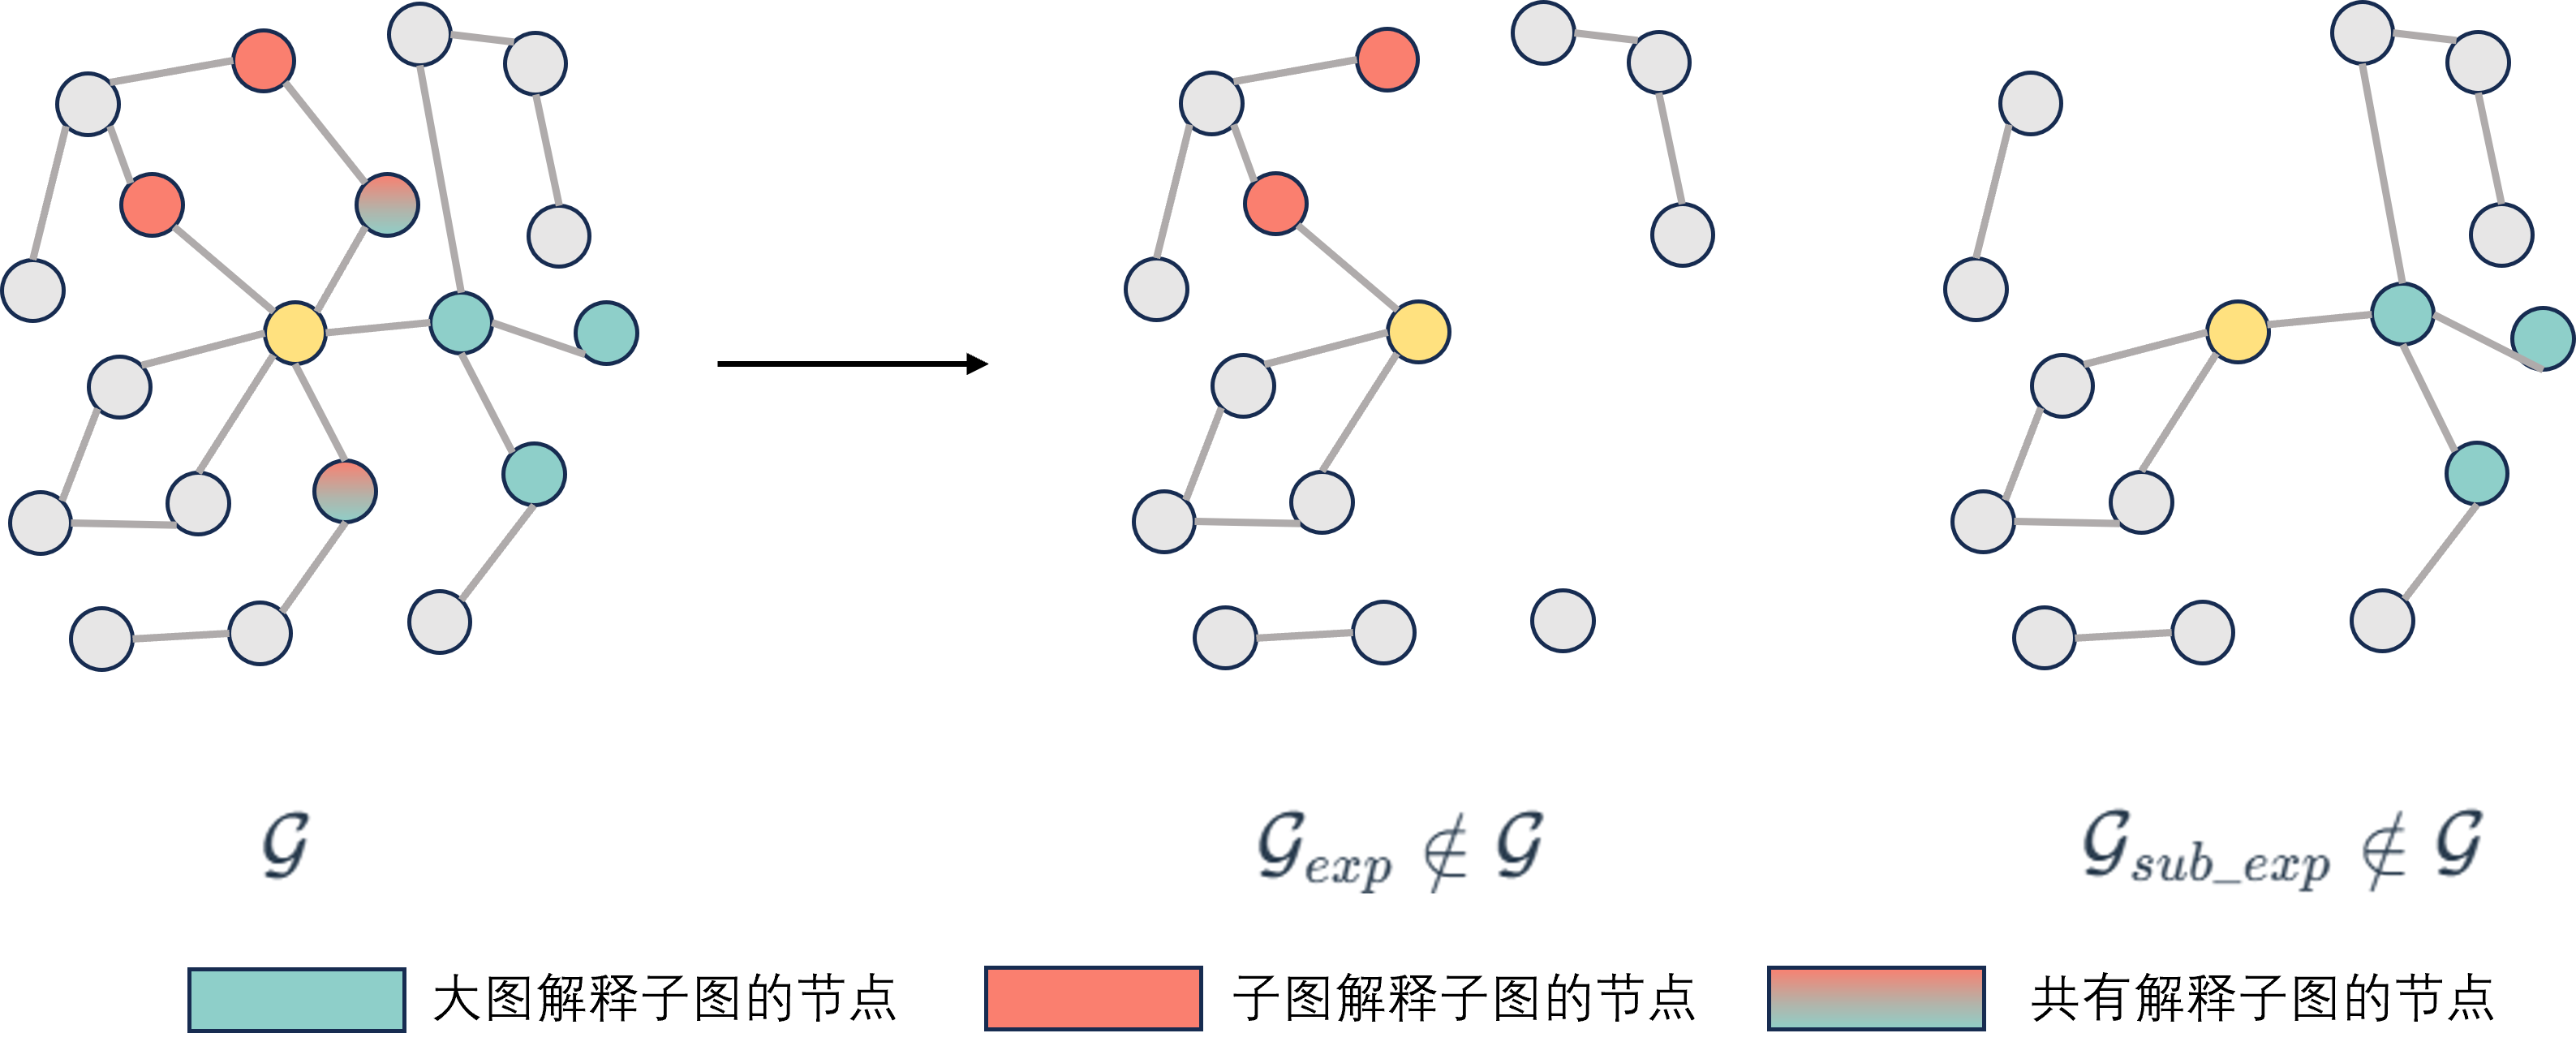
\includegraphics[width=0.8\linewidth]{pic/q3}
		\caption{评价方法示意图}
		\label{fig:99}
	\end{figure}
	

\end{frame}

\subsection{评价指标}

\begin{frame}{Fidelity评价指标}
	Fidelity(忠实度)是衡量解释模型输出与原模型输出一致性的重要指标。它通常用于评估解释模型是否能够准确反映原模型的决策过程。
\begin{block}{Fidelity数学公式}
	\begin{equation}
		\begin{aligned}
			\mathrm{fid}_{+} &= 1 - \frac{1}{N} \sum_{i=1}^N \mathbb{1}(\hat{y}_i^{G_{C\setminus S}} = \hat{y}_i) \\
			\mathrm{fid}_{-} &= 1 - \frac{1}{N} \sum_{i=1}^N \mathbb{1}(\hat{y}_i^{G_S} = \hat{y}_i)
		\end{aligned}
	\end{equation}
\end{block}

\end{frame}







	
	
	
\section{实验}
\subsection{数据集介绍}
\begin{frame}{数据集选取}
	\begin{table}[h!]
		\centering
		\caption{数据集节点数、边数及简介}
		\begin{tabularx}{\textwidth}{@{}lcccX@{}}
			\toprule[1.5pt]
			\textbf{数据集} & \textbf{节点数} & \textbf{边数} & \textbf{用途} & \textbf{特点} \\ 
			\midrule
			Citeseer     & 3,327         & 4,732        & 节点分类、链接预测 & 包含论文及其引用关系 \\ 
			Cora         & 2,708         & 5,429        & 节点分类           & 包含机器学习论文主题分类 \\ 
			PubMed       & 19,717        & 44,338       & 节点分类           & 生物医学论文与元信息 \\ 
			Reddit       & 232,965       & 11,606,919   & 图分类、社区检测   & 动态图,建模用户活动 \\ 
			ogb-products & 2,449,029     & 61,859,140   & 大规模节点分类     & OGB 提供的大规模图数据 \\ 
			\bottomrule[1.5pt]
		\end{tabularx}
		
		\label{tab:dataset_overview}
	\end{table}
\end{frame}

\subsection{实验结果}
\begin{frame}{GNNE实验结果}
\begin{table}[htbp]
	\centering
	\caption{实验结果对比}
	\begin{tabular}{cccccccccc}
		\toprule[1.5pt]
		\multirow{2}{*}{数据集} & \multirow{2}{*}{显卡} & \multicolumn{4}{c}{原始模型} & \multicolumn{4}{c}{代理模型 (Ours)} \\
		\cmidrule(lr){3-6} \cmidrule(lr){7-10}
		& & fid+ & fid- & acc & time & fid+ & fid- & acc & time \\
		\midrule
		Citeseer & 4070ti & \textbf{0.856} & 0 & 0.677 & 1:12:23 & 0.723 & 0 & 0.691 & \textbf{40:07} \\
		Cora & 4090 & 0.817 & 0 & 0.819 & 58:16
		 & \textbf{0.923} & 0 & 0.775 & \textbf{34:20} \\
		PubMed & 4090 & 0.798 & 0 & 0.793 & 5:17:23
		 & \textbf{0.851} & 0 & 0.822 & \textbf{1:34:23} \\
		Reddit & 4090 & - & - & 0.806 & -
		 & \textbf{0.862} & \textbf{0.016} & 0.834 & \textbf{3:46:52} \\
		ogb-products & 4090 & - & - & 0.736 &- & \textbf{0.846} & \textbf{0.012} & 0.798 & \textbf{21:23:10} \\
		\bottomrule[1.5pt]
	\end{tabular}
\end{table}
	
\end{frame}





\section{未来计划与安排}
\begin{frame}{未来计划与安排}
	\begin{itemize}
		\item 在更多的图神经网络解释器上进行实验。
		\item 更多的消融实验。
	\end{itemize}
\end{frame}














%==============================================================================%


%==============================================================================%


%\section{函数}


%==============================================================================%

\section*{致谢}
\kongbai
\begin{frame}
	\begin{figure}
		\centering
		
\includegraphics[width=0.9\textwidth]{CSThankyou.jpg}
	\end{figure}
	
	\footnotetext[1]{\scriptsize 本演示文稿使用 \LaTeX{} 排版工具制作,若想进一步了解这一强大的开源工具,请移步 \href{http://mirrors.cqu.edu.cn/CTAN/info/lshort/chinese/lshort-zh-cn.pdf}{\textcolor{cquptpurple}{一份(不太)简短的 \LaTeXe{} 介绍}}。}
	\footnotetext[2]{\scriptsize 在本演示文稿的制作过程中,作者从 \href{https://faculty.cqupt.edu.cn/liliu/zh_CN/index.htm}{\textcolor{cquptpurple}{重庆邮电大学~刘立}} 老师处获得了诸多指导与建议,在此表示十分感谢。}
	\footnotetext[3]{\scriptsize 感谢 \href{https://faculty.cqupt.edu.cn/lizhenkun/zh_CN/index.htm}{\textcolor{cquptpurple}{重庆邮电大学~李振坤}} 老师提供的 \LaTeX{} Beamer 模版。}
\end{frame}


\end{document} 